% This is the Reed College LaTeX thesis template. Most of the work 
% for the document class was done by Sam Noble (SN), as well as this
% template. Later comments etc. by Ben Salzberg (BTS). Additional
% restructuring and APA support by Jess Youngberg (JY).
% Your comments and suggestions are more than welcome; please email
% them to cus@reed.edu
%
% See http://web.reed.edu/cis/help/latex.html for help. There are a 
% great bunch of help pages there, with notes on
% getting started, bibtex, etc. Go there and read it if you're not
% already familiar with LaTeX.
%
% Any line that starts with a percent symbol is a comment. 
% They won't show up in the document, and are useful for notes 
% to yourself and explaining commands. 
% Commenting also removes a line from the document; 
% very handy for troubleshooting problems. -BTS

% As far as I know, this follows the requirements laid out in 
% the 2002-2003 Senior Handbook. Ask a librarian to check the 
% document before binding. -SN

%%
%% Preamble
%%
% \documentclass{<something>} must begin each LaTeX document
\documentclass[12pt,twoside]{reedthesis}
% Packages are extensions to the basic LaTeX functions. Whatever you
% want to typeset, there is probably a package out there for it.
% Chemistry (chemtex), screenplays, you name it.
% Check out CTAN to see: http://www.ctan.org/
%%
\usepackage{graphicx,latexsym} 
\usepackage{amssymb,amsthm,amsmath}
\usepackage{longtable,booktabs,setspace} 
\usepackage{chemarr} %% Useful for one reaction arrow, useless if you're not a chem major
\usepackage[hyphens]{url}
\usepackage{rotating}
\usepackage{natbib}
% Comment out the natbib line above and uncomment the following two lines to use the new 
% biblatex-chicago style, for Chicago A. Also make some changes at the end where the 
% bibliography is included. 
%\usepackage{biblatex-chicago}
%\bibliography{thesis}

% \usepackage{times} % other fonts are available like times, bookman, charter, palatino

\title{Empirical Analysis of Fair Hierarchical Clustering Algorithms}
\author{Param Kapur}
% The month and year that you submit your FINAL draft TO THE LIBRARY (May or December)
\date{December 2025}
\division{Mathematical and Natural Sciences}
\advisor{Harper Knittel}
%If you have two advisors for some reason, you can use the following
%\altadvisor{Your Other Advisor}
%%% Remember to use the correct department!
\department{Computer Science}
% if you're writing a thesis in an interdisciplinary major,
% uncomment the line below and change the text as appropriate.
% check the Senior Handbook if unsure.
%\thedivisionof{The Established Interdisciplinary Committee for}
% if you want the approval page to say "Approved for the Committee",
% uncomment the next line
%\approvedforthe{Committee}

\setlength{\parskip}{0pt}
%%
%% End Preamble
%%
%% The fun begins:
\begin{document}

  \maketitle
  \frontmatter % this stuff will be roman-numbered
  \pagestyle{empty} % this removes page numbers from the frontmatter

% Acknowledgements (Acceptable American spelling) are optional
% So are Acknowledgments (proper English spelling)
    \chapter*{Acknowledgements}
	I want to thank a few people.

% The preface is optional
% To remove it, comment it out or delete it.
    \chapter*{Preface}
	This is an example of a thesis setup to use the reed thesis document class.
	
	

    \chapter*{List of Abbreviations}
		You can always change the way your abbreviations are formatted. Play around with it yourself, use tables, or come to CUS if you'd like to change the way it looks. You can also completely remove this chapter if you have no need for a list of abbreviations. Here is an example of what this could look like:

	\begin{table}[h]
	\centering % You could remove this to move table to the left
	\begin{tabular}{ll}
		\textbf{ABC}  	&  American Broadcasting Company \\
		\textbf{CBS}  	&  Columbia Broadcasting System\\
		\textbf{CDC}  	&  Center for Disease Control \\
		\textbf{CIA}  	&  Central Intelligence Agency\\
		\textbf{CLBR} 	&  Center for Life Beyond Reed\\
		\textbf{CUS}  	&  Computer User Services\\
		\textbf{FBI}  	&  Federal Bureau of Investigation\\
		\textbf{NBC}  	&  National Broadcasting Corporation\\
	\end{tabular}
	\end{table}
	

    \tableofcontents
% if you want a list of tables, optional
    \listoftables
% if you want a list of figures, also optional
    \listoffigures

% The abstract is not required if you're writing a creative thesis (but aren't they all?)
% If your abstract is longer than a page, there may be a formatting issue.
    \chapter*{Abstract}
	The preface pretty much says it all.
	
	\chapter*{Dedication}
	You can have a dedication here if you wish.

  \mainmatter % here the regular arabic numbering starts
  \pagestyle{fancyplain} % turns page numbering back on

%The \introduction command is provided as a convenience.
%if you want special chapter formatting, you'll probably want to avoid using it altogether

    \chapter*{Introduction}
         \addcontentsline{toc}{chapter}{Introduction}
	\chaptermark{Introduction}
	\markboth{Introduction}{Introduction}
	% The three lines above are to make sure that the headers are right, that the intro gets included in the table of contents, and that it doesn't get numbered 1 so that chapter one is 1.

% Double spacing: if you want to double space, or one and a half 
% space, uncomment one of the following lines. You can go back to 
% single spacing with the \singlespacing command.
% \onehalfspacing
% \doublespacing
	
	Welcome to the \LaTeX\ thesis template. If you've never used \TeX\ or \LaTeX\ before, you'll have an initial learning period to go through, but the results of a nicely formatted thesis are worth it for more than the aesthetic benefit: markup like \LaTeX\ is more consistent than the output of a word processor, much less prone to corruption or crashing and the resulting file is smaller than a Word file. While you may have never had problems using Word in the past, your thesis is going to be about twice as large and complex as anything you've written before, taxing Word's capabilities. If you're still on the fence about  using \LaTeX, read the Introduction to LaTeX on the CUS site as well as skim the following template and give it a few weeks. Pretty soon all the markup gibberish will become second nature.

\section{Why use it?}
	
\LaTeX\ does a great job of formatting tables and paragraphs. Its line-breaking algorithm was the subject of a PhD.\thinspace thesis. It does a fine job of automatically inserting ligatures, and to top it all off it is the only way to typeset good-looking mathematics.

\section{Who should use it?}

Anyone who needs to use math, tables, a lot of figures, complex cross-references, IPA or who just cares about the final appearance of their document should use \LaTeX. At Reed, math majors are required to use it, most physics majors will want to use it, and many other science majors may want it also.
	
\chapter{Background}
	This is the first page of the first chapter. You may delete the contents of this chapter so you can add your own text; it's just here to show you some examples. 
	\section{Hierarchical Clustering and Cost}
	\subsection{Definition and Concepts}
		**Definition**: Hierarchical clustering is an unsupervised learning method that produces a hierarchy of nested clusters organized in a tree structure (dendrogram). Formally, it can be represented as a binary tree $T$ whose leaves correspond to individual data points in dataset $X$ and whose internal nodes represent merged clusters containing those points. Each level of the tree yields a different partition of the data.

	\subsection{Cost Functions in Hierarchical Clustering}
		Dasguptaaa


	\section{Fairness Concepts in Machine Learning}\label{sec:fairness_concepts}
		Machine learning has fundamentally transformed decision-making by
allowing algorithms to discover intricate and
meaningful patterns directly from data, without relying explicitly on
predefined rules. Rather than encoding
human expertise through manual programming, machine learning
algorithms generalize from examples. This inductive
process, which generalizes observed cases to unseen scenarios,
enables the algorithm to identify underlying patterns
from historical examples and predict future outcomes. However, such a
reliance on historical data inherently carries
risks, especially when data reflects existing societal biases,
stereotypes, or inequalities.

\subsection{Algorithmic Bias}\label{subsec:algorithmic_bias}

Algorithmic bias refers to systematic and repeatable errors or unfair
outcomes produced by machine learning models
due to biases embedded within the training data or algorithm design.
According to existing literature
\cite{barocas2016big,pessach2020algorithmic}, algorithmic bias
commonly originates from:

\begin{itemize}
  \item \textbf{Biases inherent in training datasets:} These biases
    result from biased human decisions, measurement errors,
    reporting inaccuracies, or historical prejudices embedded in
    datasets. Machine learning algorithms, aiming at optimizing
    prediction accuracy, often replicate these biases.
  \item \textbf{Biases due to missing data:} When datasets lack
    sufficient representation from certain groups or have
    significant data omissions, the resulting models fail to
    accurately represent the target population.
  \item \textbf{Algorithmic optimization bias:} Typical optimization
    objectives, such as minimizing aggregate prediction
    errors, tend to favor majority groups, often leading to poorer
    performance for minority groups.
  \item \textbf{Bias from proxy attributes:} Non-sensitive attributes
    may indirectly capture sensitive information
    (e.g., race, gender, age), unintentionally introducing biases
    even when sensitive attributes are explicitly excluded
    from the dataset.
\end{itemize}

\subsection{Defining Fairness in Machine
Learning}\label{subsec:fairness_definitions}

Given the increasing use of machine learning in high-stakes domains,
rigorous fairness definitions have emerged to guide
algorithmic development. These definitions typically fall into two
broad categories: individual fairness and group fairness.

\paragraph{Individual Fairness.}
Individual fairness requires models to produce similar outputs for
similar individuals, where similarity is assessed based
on relevant non-sensitive features. Formally, individual fairness can
be articulated using Lipschitz continuity
as follows \cite{dwork2012fairness}:
\[
  d(\text{output}(x), \text{output}(x')) \leq \rho \cdot d(x, x'),
\]
where \(x\) and \(x'\) are individuals with comparable non-sensitive
attributes, and \(\rho\) is a small constant. This definition
emphasizes the fair treatment of similar cases on an individual
basis, ensuring minimal unjustified variability.

\paragraph{Group Fairness.}
Group fairness demands that statistical outcomes of algorithms be
equitable across predefined demographic groups.
This approach explicitly acknowledges and attempts to rectify
societal disparities. Notable metrics
for group fairness include:

\begin{itemize}
  \item \textbf{Demographic Parity:} Ensures equal rates of positive
    predictions across demographic groups:
    \[
      P(R = 1 \mid A = a) = P(R = 1 \mid A = b),
    \]
    where \(R\) denotes the model's prediction and \(A\) represents a
    protected attribute (e.g., race, gender).

  \item \textbf{Equal Opportunity:} Requires equal true positive
    rates among groups, ensuring fairness in the
    allocation of positive outcomes given actual positives:
    \[
      P(R = 1 \mid Y = 1, A = a) = P(R = 1 \mid Y = 1, A = b),
    \]
    with \(Y\) representing the true outcome.

  \item \textbf{Equalized Odds:} Further requires equal true positive
    and false positive rates across groups,
    encompassing both success and error equity:
    \[
      P(R = 1 \mid Y = y, A = a) = P(R = 1 \mid Y = y, A = b), \quad
      \forall y \in \{0, 1\}.
    \]
\end{itemize}

Each of these metrics presents trade-offs, and no universal criterion
exists to satisfy all simultaneously,
leading to a fundamental tension explored later.

\subsection{Real-World Instances and Ethical Dimensions of
Algorithmic Bias}\label{subsec:real_world_bias}

Concrete examples vividly illustrate the risks associated with biased
algorithms. One widely cited example is the COMPAS algorithm,
frequently used in criminal justice for predicting recidivism.
Investigations revealed significant racial biases, incorrectly
labeling Black defendants as high-risk at nearly twice the rate of
White defendants who later re-offended~\cite{angwin2016machine}.
Similarly, facial recognition software has consistently demonstrated
higher error rates for darker-skinned individuals, exacerbating risks
of racial profiling and wrongful identification.

Algorithmic biases also permeate employment contexts, where
historical data reflecting past hiring decisions embed biases against
women or minority groups, perpetuating discrimination through
ostensibly neutral automated decision-making systems. When training
algorithms on historical employment records, biases and stereotypes
embedded in the data disproportionately disadvantage female candidates.

A particularly telling example emerges from machine translation.
Consider translating sentences from English to Turkish and then back
into English, as illustrated in Figures~\ref{fig:eng-to-turkish}
and~\ref{fig:turkish-to-eng}. Turkish pronouns are gender-neutral,
but when translated back into English, gender-specific pronouns are
inferred based on statistical associations. As a result, occupations
stereotypically associated with men—such as ``engineer'' or
``doctor''—are translated back using male pronouns, while occupations
stereotypically associated with women—such as ``nurse''—return female
pronouns. This phenomenon arises from two biases embedded in training
datasets: real-world labor market statistics reflecting historical
occupational distributions and the ``male-as-norm'' bias, whereby
male pronouns are preferentially selected when gender is ambiguous or
unknown~\cite{caliskan2017semantics}.

\begin{figure}[h]
  \centering
  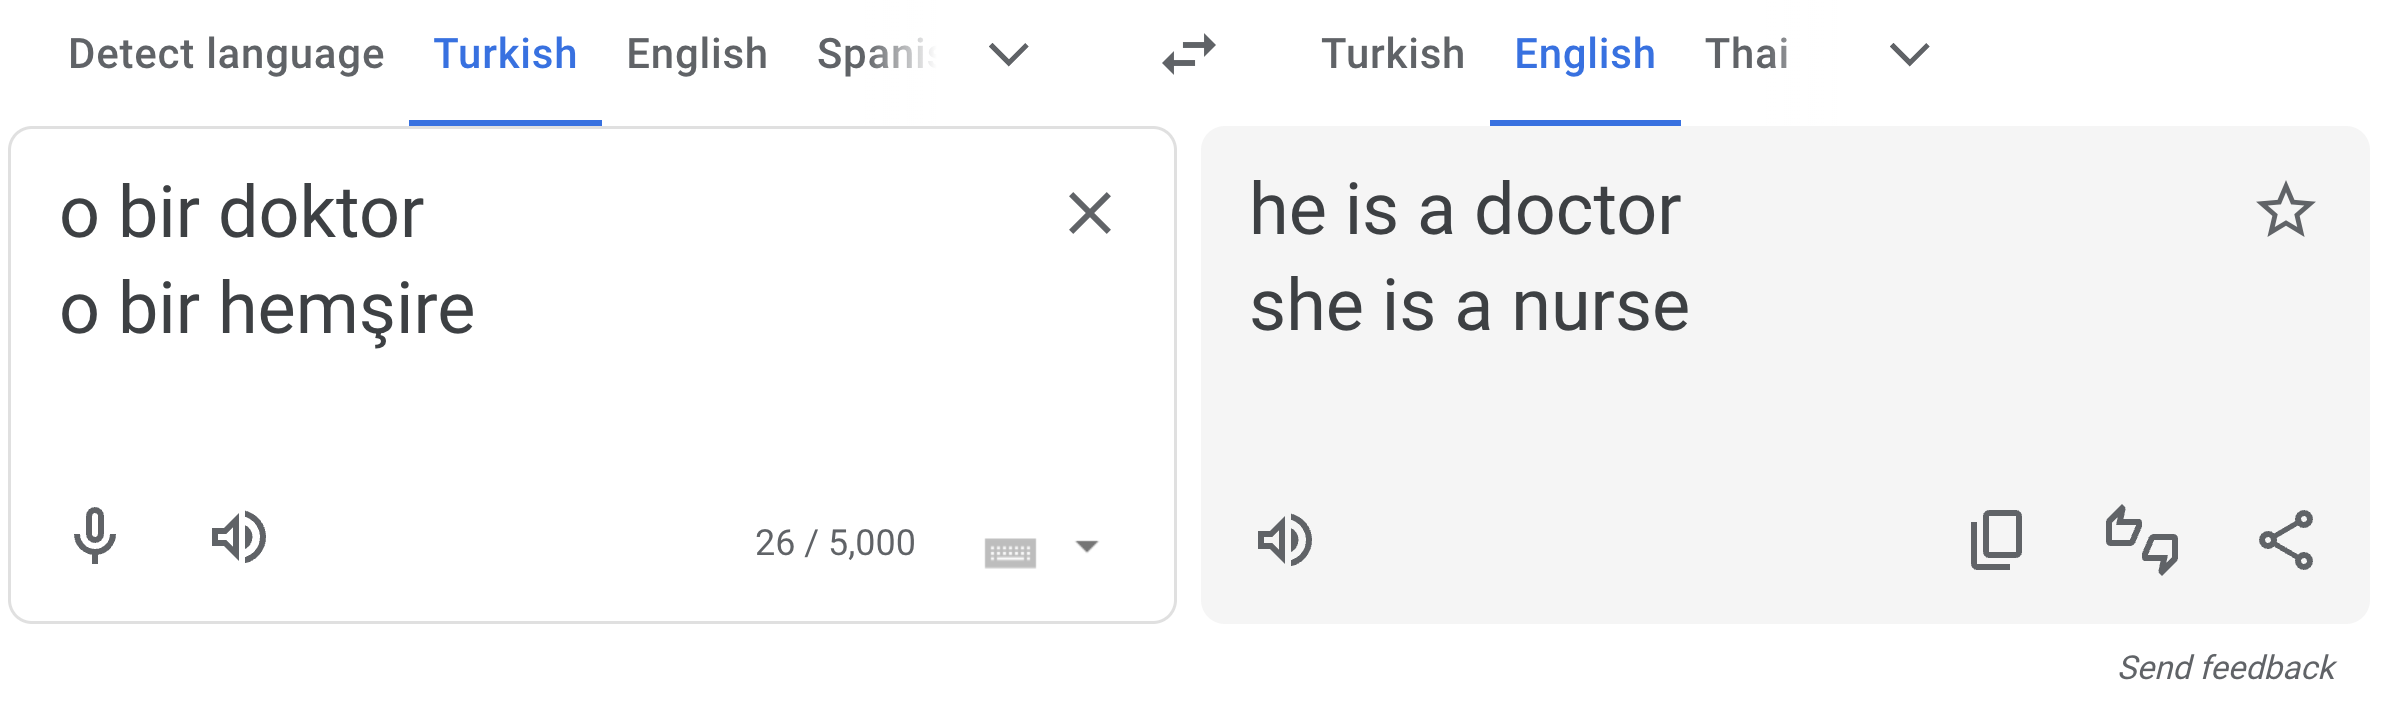
\includegraphics[width=0.9\textwidth]{sections/background/turkish-to-eng.png}
  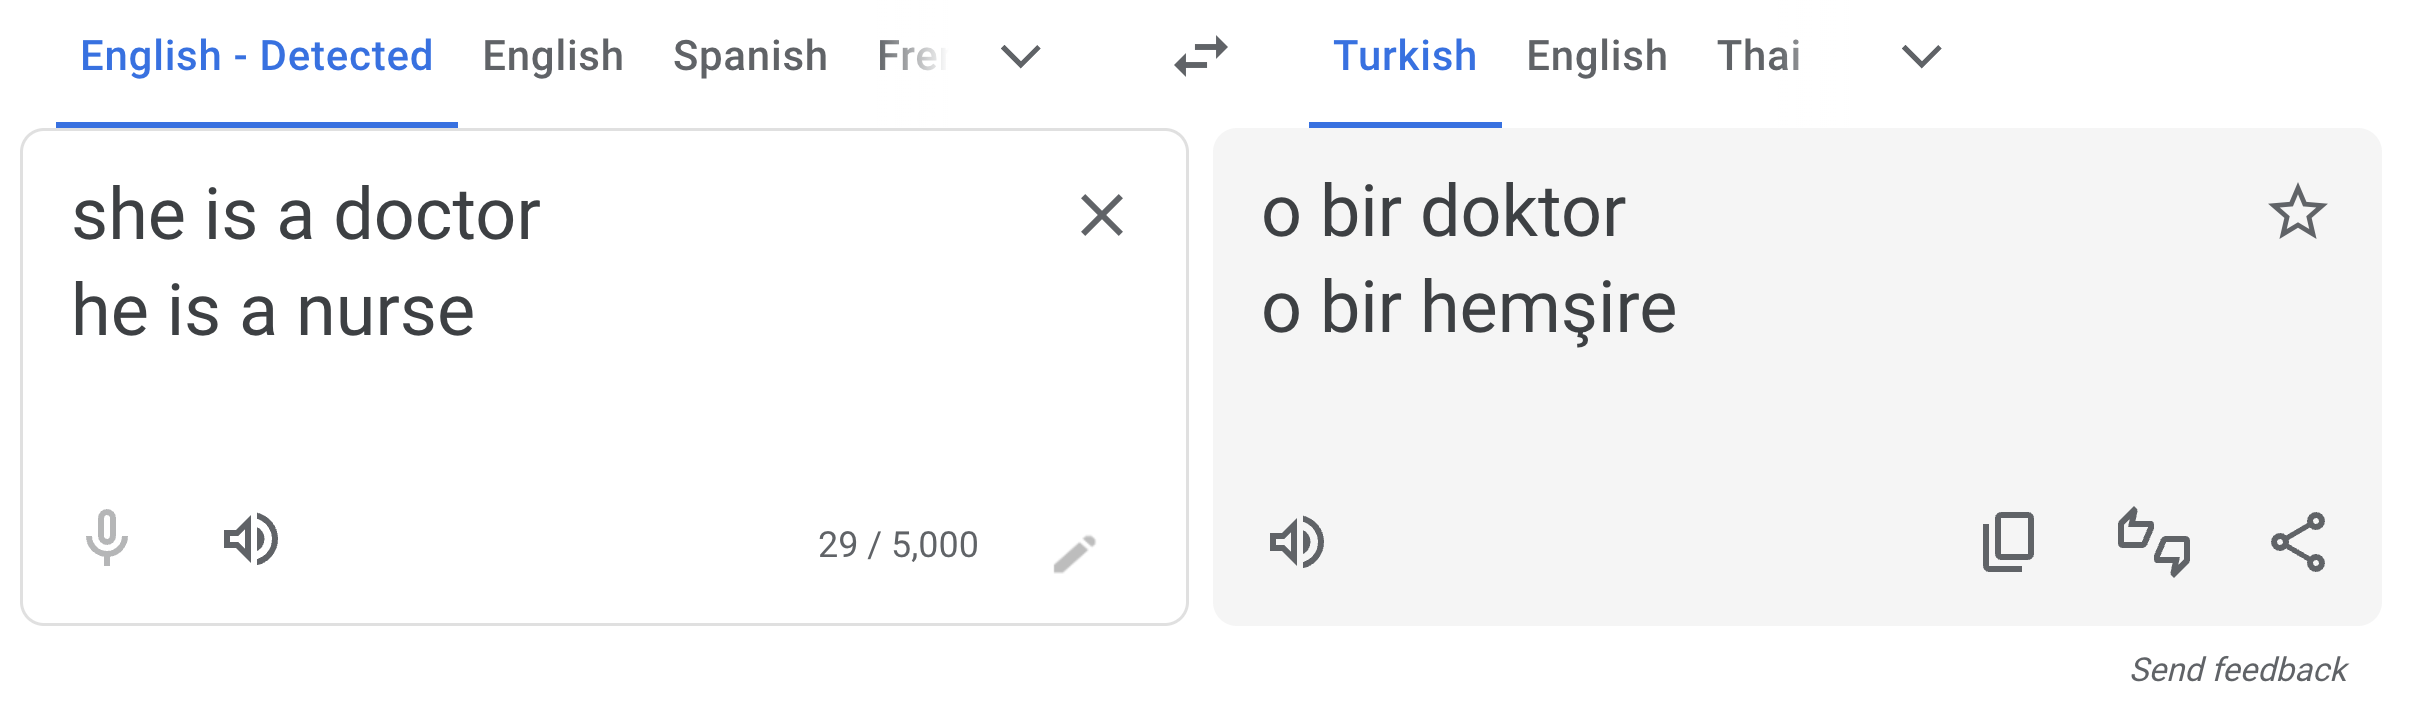
\includegraphics[width=0.9\textwidth]{sections/background/eng-to-turkish.png}
  \caption{Translations of gender-specific English sentences into
  gender-neutral Turkish and then back to English.}
  \label{fig:eng-to-turkish}
\end{figure}

Attempts to mitigate biases by removing explicitly sensitive
attributes (such as gender or race) from training datasets frequently
fall short due to \textit{proxy variables}. Proxy attributes—such as
the age at which individuals start programming—can inadvertently
encode sensitive information like gender, reinforcing biases even in
their absence. Additionally, biases due to disparities in sample
sizes among demographic groups lead to poorer model performance for
minority groups, reinforcing systematic inequities~\cite{barocas2016big}.

Beyond technical considerations, fairness intersects profoundly with
ethical and legal imperatives. Legal frameworks such as Title VII of
the U.S. Civil Rights Act mandate nondiscrimination in employment.
Similarly, regulatory initiatives like the European Union’s GDPR and
proposed AI Act embed fairness, transparency, and equity into
regulatory requirements for algorithmic systems.

Ethically, ensuring fairness aligns closely with broader principles
of justice and equity, particularly as algorithmic systems
increasingly influence societal outcomes such as employment,
education, and criminal justice. Effective fairness interventions
help prevent reinforcing historical injustices, foster social equity,
and maintain public trust in algorithm-driven decision-making.

\subsection{Challenges, Limitations, and Future
Directions}\label{subsec:challenges_future}
(TODO: citations here need to be filled in carefully I relied a bit
on yt tAjFuhkiV2c)

The growing emphasis on fairness in algorithmic decision-making,
particularly in clustering and machine learning contexts, has
significantly advanced our understanding of bias mitigation.
Nevertheless, this field continues to face considerable challenges
and inherent limitations.

One prominent difficulty arises from conflicting fairness criteria.
It is mathematically impossible to simultaneously satisfy all
fairness definitions—such as Demographic Parity, Equal Opportunity,
and Equalized Odds—highlighting the necessity for context-specific
fairness solutions. For example, attempts to apply broad fairness
concepts, initially developed within supervised learning frameworks,
to clustering tasks often encounter mismatches in meaning. Individual
fairness definitions emphasizing distributional equity may not
translate effectively into clustering contexts, where groups or
clusters often lack inherent meaning until assigned. This mismatch
underscores the need to carefully adapt fairness criteria from
supervised learning to unsupervised scenarios.

Moreover, algorithmic fairness interventions rarely function in
isolation. They typically constitute components within broader
socio-technical systems, necessitating careful consideration of both
upstream inputs and downstream impacts. The removal of sensitive
variables, a common fairness strategy, can inadvertently lead to
unintended consequences. For instance, the practice of "Ban the Box,"
intended to eliminate employment discrimination by prohibiting
questions about criminal history, inadvertently increased racial
discrimination as employers began using race as a proxy variable.
This underscores the complexity and potential pitfalls inherent in
algorithmic fairness interventions and highlights the importance of
anticipating and managing unintended downstream consequences.

Further complications emerge from the dynamic nature of real-world
data. In applications such as school districting or political
redistricting, clustering algorithms are applied to dynamic
populations, where individuals may relocate in response to
algorithmic interventions. Historical efforts like school busing
aimed at integrating racially segregated districts illustrate how
algorithmic clustering solutions can unintentionally disrupt
communities or exacerbate segregation through mechanisms such as
"white flight." This historical context reveals the critical need to
engage deeply with domain-specific constraints, legal frameworks, and
stakeholder needs, reinforcing that algorithmic solutions must be
cognizant of broader historical and societal dynamics.

Indeed, addressing these multidimensional challenges requires
interdisciplinary collaboration beyond computer science. Integrating
insights from fields such as sociology, criminology, economics, law,
and ethics is critical. For instance, fairness research often
overlooks valuable contributions from disciplines like criminology or
education policy, which provide nuanced understandings of systemic
inequities and practical constraints. Collaboration with experts from
these domains can guide the appropriate adaptation of algorithmic
methods to complex social contexts, ensuring solutions align closely
with practical realities and ethical standards.

Another essential consideration is stakeholder engagement. Too often,
fairness solutions are developed paternalistically, without
adequately involving those directly impacted. Engaging
stakeholders—including affected communities, policy experts, and
practitioners—in defining fairness and assessing interventions can
prevent misguided assumptions and ensure that algorithmic systems
genuinely serve intended beneficiaries. This is particularly evident
in sensitive domains such as criminal justice, healthcare, and
education, where the risk of inadvertently causing harm or
perpetuating injustices remains high.

Finally, reliance on commonly used benchmark datasets, such as the
COMPAS, Adult, and German Credit datasets, introduces risks of
replicating inherent data biases and inaccuracies. Issues such as
noisy demographic labels, inappropriate or misleading features, and
the misalignment of fairness labels highlight critical weaknesses in
the existing empirical evaluation landscape. Consequently, rigorous
methodological scrutiny and the development of better benchmarks
reflecting real-world complexities and accurate demographic
information are urgently needed.

In summary, future directions in algorithmic fairness research must
navigate inherent mathematical and practical complexities through
rigorous interdisciplinary collaboration, careful stakeholder
engagement, and meticulous empirical practices. By integrating
technical algorithmic approaches with broader societal, legal, and
ethical considerations, researchers can develop more robust,
equitable, and practically viable solutions to mitigate algorithmic
biases and their profound societal implications.




\chapter*{Conclusion}
         \addcontentsline{toc}{chapter}{Conclusion}
	\chaptermark{Conclusion}
	\markboth{Conclusion}{Conclusion}
	\setcounter{chapter}{4}
	\setcounter{section}{0}
	
Here's a conclusion, demonstrating the use of all that manual incrementing and table of contents adding that has to happen if you use the starred form of the chapter command. The deal is, the chapter command in \LaTeX\ does a lot of things: it increments the chapter counter, it resets the section counter to zero, it puts the name of the chapter into the table of contents and the running headers, and probably some other stuff. 

So, if you remove all that stuff because you don't like it to say ``Chapter 4: Conclusion'', then you have to manually add all the things \LaTeX\ would normally do for you. Maybe someday we'll write a new chapter macro that doesn't add ``Chapter X'' to the beginning of every chapter title.

\section{More info}
And here's some other random info: the first paragraph after a chapter title or section head \emph{shouldn't be} indented, because indents are to tell the reader that you're starting a new paragraph. Since that's obvious after a chapter or section title, proper typesetting doesn't add an indent there. 


%If you feel it necessary to include an appendix, it goes here.
    \appendix
      \chapter{The First Appendix}
      \chapter{The Second Appendix, for Fun}


%This is where endnotes are supposed to go, if you have them.
%I have no idea how endnotes work with LaTeX.

  \backmatter % backmatter makes the index and bibliography appear properly in the t.o.c...

% if you're using bibtex, the next line forces every entry in the bibtex file to be included
% in your bibliography, regardless of whether or not you've cited it in the thesis.
    \nocite{*}

% Rename my bibliography to be called "Works Cited" and not "References" or ``Bibliography''
% \renewcommand{\bibname}{Works Cited}

%    \bibliographystyle{bsts/mla-good} % there are a variety of styles available; 
%  \bibliographystyle{plainnat}
% replace ``plainnat'' with the style of choice. You can refer to files in the bsts or APA 
% subfolder, e.g. 
 \bibliographystyle{APA/apa-good}  % or
 \bibliography{thesis}
 % Comment the above two lines and uncomment the next line to use biblatex-chicago.
 %\printbibliography[heading=bibintoc]

% Finally, an index would go here... but it is also optional.
\end{document}
